\documentclass[a4paper]{article}
\usepackage{xgreek}
\usepackage{xltxtra}
\usepackage{graphics}
\setlength{\topmargin}{0in}
\setlength{\oddsidemargin}{0in}
\setlength{\evensidemargin}{0in}
\setlength{\textheight}{9in}
\setlength{\textwidth}{6.25in}
\setmainfont[Mapping=tex-text]{GFS Didot}

\begin{document}
\section{Κονσόλα Διαχείρισης Κόμβων}
Η κονσόλα διαχείρισης κόμβων του ScorpioFS είναι μια λειτουργία με την οποία
μπορούμε να διαχειριστούμε μαζικά και απομακρυσμένα κόμβους του δικτύου.
Χρησιμοποιείται για την γρήγορη και εύκολη εκτέλεση πειραμάτων σε περιβάλλον
εργαστηρίου με σκοπό την εξαγωγή διάφορων στατιστικών στοιχείων. Όπως
φαίνεται και στο Σχήμα \ref{fig:topology}, το δίκτυο αποτελείται από τους Chord
κόμβους, όπου κάθε ένας έχει ένα proxy server για να επικοινωνεί με την κονσόλα,
ένα μηχάνημα με το σύστημα ScorpioFS στο οποίο υπάρχει και η κονσόλα
διαχείρισης. Κάθε μηχάνημα μπορεί να γίνει και κόμβος του Chord δικτύου. Στο
Σχήμα \ref{fig:topology} το μηχάνημα που τρέχει το ScorpioFS σύστημα και την
κονσόλα δεν είναι κόμβος του Chord δικτύου για λόγους απλοποίησης του σχήματος
και καλύτερης κατανόησής του.

\begin{figure}[tbh]
\centering
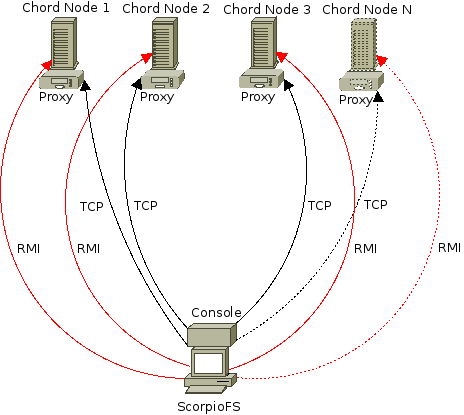
\includegraphics[scale=0.75]{images/scorpio_console.png}
\caption{Τοπολογία δικτύου κόμβων}
\label{fig:topology}
\end{figure}

Για λόγους αποδοτικότητας αποφύγαμε τις κλήσεις \emph{RMI} μεταξύ της κονσόλας
διαχείρισης και των κόμβων του δικτύου. Όλη η ανταλλαγή μηνυμάτων γίνεται με το
πρωτόκολλο \emph{TCP} και sockets. Για το λόγο αυτό κάθε κόμβος έχει ένα
διαδικτυακό μεσολαβητή (proxy
server) ο οποίος δέχεται και στέλνει \emph{TCP} μηνύματα από τη κονσόλα και αυτός 
είναι υπεύθυνος για τις \emph{RMI} κλήσεις που χρειάζονται. Με αυτό τον τρόπο δεν
επιβαρύνεται η κονσόλα με πολλαπλές ανταλλαγές μηνυμάτων μέσω του πρωτοκόλλου
\emph{RMI}. Τα \emph{TCP} μηνύματα που ανταλλάσσονται είναι σε μορφή κειμένου και
η κωδικοποίηση που χρησιμοποιείται είναι η default κωδικοποίηση που χρησιμοποιεί το
Java Runtine Enviroment. Η default κωδικοποίηση των μηχανημάτων στα εργαστήρια
είναι \emph{US-ASCII}.

\subsection{Επικοινωνία κονσόλας προς κόμβους}
Ο TCP server στον proxy κάθε Chord κόμβου ακούει στη πόρτα 6789 για εισερχόμενα
μηνύματα. Ανάλογα με τις εντολές που έχει δώσει ο χρήστης τα μηνύματα μπορεί να
είναι είτε για το ξεκίνημα κάποιου κόμβου, είτε για το σταμάτημα κάποιου κόμβου,
είτε για την παραγωγή στατιστικών για κάποιο κόμβο. Αφού σταλεί το μήνυμα,
κλείνει η TCP σύνδεση μεταξύ κονσόλας και proxy, και ο τελευταίος κάνει τις
κατάλληλες RMI κλήσεις. Το πρωτόκολλο επικοινωνίας είναι το παρακάτω:
\begin{enumerate}
\item \textbf{Κωδικός Λειτουργίας (OP Code)} -- Ο κωδικός που αντιστοιχεί σε
λειτουργία. Αναλυτικά στον Πίνακα \ref{tab:opcodes}.
\item \textbf{Πόρτα Λειτουργίας} -- Η πόρτα που θα λειτουργεί ο Chord κόμβος.
\item \textbf{Αρχείο Ρυθμίσεων} -- Το αρχείο παραμετροποίησης που θα
χρησιμοποιηθεί για το συγκεκριμένο κόμβο.
\end{enumerate}

Η default πόρτα λειτουργίας ενός κόμβου είναι η 6788. Σε περίπτωση όμως που η
πόρτα αυτή είναι δεσμευμένη από κάποια άλλη εφαρμογή μπορούμε να ορίσουμε
διαφορετική πόρτα λειτουργίας. Το Αρχείο Ρυθμίσεων περιέχει ρυθμίσεις για
τη σωστή λειτουργία του κόμβου. Ανάλογα με το στήσιμο του δικτύου μπορεί να
χρειαστεί να αλλάξει. Για παράδειγμα όταν τρέχουν δύο κόμβοι στο ίδιο μηχάνημα,
θα πρέπει να έχουν διαφορετικό αρχείο ρυθμίσεων. Ο ένας θα έχει το default και ο
άλλος διαφορετικό που θα πρέπει να το δηλώσουμε explicit.

\begin{table}[h!b!p!]
\begin{center}
\begin{tabular}{| c | c | c |}
\hline
\textbf{Mnemonics} & \textbf{OP Code} & \textbf{Operation}\\
\hline
\hline
NODE\_CREATE & 0 & Δημιουργία ενός κόμβου\\
\hline
NODE\_STOP & 1 & Σταμάτημα ενός κόμβου\\
\hline
NODE\_STAT & 2 & Συγκέντρωση στατιστικών για ένα κόμβο\\
\hline
\end{tabular}
\end{center}
\caption{Λειτουργίες και οι κωδικοί τους}
\label{tab:opcodes}
\end{table}

\subsection{Επικοινωνία κόμβων προς κονσόλα}
Η κονσόλα διαχείρισης δέχεται και αυτή μηνύματα από τους κόμβους. Για το λόγο
αυτό έχει υλοποιηθεί και στην κονσόλα ένας TCP server στην πόρτα 7891. Τα
μηνύματα που δέχεται η κονσόλα από τους κόμβους του Chord δικτύου μπορούν να
χωριστούν σε δύο κατηγορίες.

Η πρώτη κατηγορία είναι τα μηνύματα επιβεβαίωσης από τους κόμβους για τις
διάφορες λειτουργίες. Δηλαδή για κάθε λειτουργία που στέλνει αρχικά η κονσόλα
προς κάποιο κόμβο, περιμένει και ένα μήνυμα επιβεβαίωσης. Για παράδειγμα όταν
δοθεί η εντολή για την εκκίνηση κάποιου κόμβου, η κονσόλα στέλνει την εντολή στο
συγκεκριμένο κόμβο και έπειτα ο κόμβος στέλνει ένα μήνυμα στην κονσόλα. Το
μήνυμα μπορεί να είναι επιτυχίας ή αποτυχίας.

Το πρωτόκολλο που χρησιμοποιείται για την αποστολή των μηνυμάτων επιβεβαίωσης
είναι το παρακάτω:
\begin{enumerate}
\item \textbf{Πόρτα λειτουργίας proxy} -- Η πόρτα λειτουργίας του proxy server
από τον οποίο στάλθηκε το μήνυμα.
\item \textbf{Μήνυμα} -- Το μήνυμα επιστροφής υπό τη μορφή κάποιου κωδικού.
Αναλυτικά στον Πίνακα \ref{tab:messages}.
\item \textbf{Πόρτα λειτουργίας κόμβου} -- Η πόρτα λειτουργίας του Chord κόμβου
για τον οποίο αναφέρεται το μήνυμα.
\end{enumerate}

\begin{table}[h!b!p!]
\begin{center}
\begin{tabular}{| c | c | c |}
\hline
\textbf{Μnemonics} & \textbf{OP Code} & \textbf{Message}\\
\hline
\hline
CREATED & 8 & Ο κόμβος ξεκίνησε επιτυχώς.\\
\hline
NOT\_CREATED & 9 & Ο κόμβος δεν ξεκίνησε.\\
\hline
STOPPED & 10 & Ο κόμβος σταμάτησε επιτυχώς.\\
\hline
NOT\_STOPPED & 11 & Ο κόμβος δεν σταμάτησε.\\
\hline
\end{tabular}
\end{center}
\caption{Μηνύματα επιβεβαίωσης και οι κωδικοί τους}
\label{tab:messages}
\end{table}

Η άλλη κατηγορία μηνυμάτων που στέλνονται στην κονσόλα διαχείρισης είναι τα
στατιστικά. Το \emph{ScorpioFS} έχει τη δυνατότητα να συλλέξει κάποια στοιχεία από
τους κόμβους του δικτύου του για την παραγωγή στατιστικών. Τα στατιστικά που μας
ενδιαφέρουν είναι το πλήθος των αιτήσεων που έχει δεχθεί ένας κόμβος για την
αποθήκευση δεδομένων, το πλήθος των αιτήσεων που έχει δεχθεί ένας
κόμβος για ανάκτηση δεδομένων και το μέγεθος των δεδομένων που έχει
αποθηκευμένα.

Για το λόγο αυτό εκτός από τα μηνύματα που ήδη αναφέραμε, σε αυτή την
περίπτωση στέλνονται και τα παρακάτω:
\begin{enumerate}
\item Πλήθος αιτήσεων για αποθήκευση δεδομένων.
\item Πλήθος αιτήσεων για ανάκτηση δεδομένων.
\item Μέγεθος δεδομένων που έχει αποθηκευμένα ο κόμβος.
\end{enumerate}

Και στις δύο περιπτώσεις μετά την αποστολή ενός πακέτου μηνυμάτων, κλείνει η
σύνδεση μεταξύ ενός κόμβου και της κονσόλας διαχείρισης.
\end{document}
